\documentclass[conference]{IEEEtran}
\IEEEoverridecommandlockouts
% The preceding line is only needed to identify funding in the first footnote. If that is unneeded, please comment it out.
\usepackage{cite}
\usepackage{amsmath,amssymb,amsfonts}
\usepackage{algorithmic}
\usepackage{graphicx}
\usepackage{textcomp}
\usepackage{xcolor}
\def\BibTeX{{\rm B\kern-.05em{\sc i\kern-.025em b}\kern-.08em
    T\kern-.1667em\lower.7ex\hbox{E}\kern-.125emX}}
\begin{document}

\title{Brain ViT: Multi-Label Classification of Brain Pathologies using Vision Transformers \\
}

\author{\IEEEauthorblockN{Sony Reddy Gurram}
\IEEEauthorblockA{\textit{University of South Dakota} \\
Vermillion, SD\\
SonyReddy.Gurram@coyotes.usd.edu}
\and
\IEEEauthorblockN{Sainath Vaddi}
\IEEEauthorblockA{\textit{University of South Dakota} \\
Vermillion, SD\\
Sainath.Vaddi@coyotes.usd.edu}
\and
\IEEEauthorblockN{Neerajdattu Dattum}
\IEEEauthorblockA{\textit{University of South Dakota} \\
Vermillion, SD \\
Neerajdattu.Dattum@coyotes.usd.edu}
\and
\IEEEauthorblockN{Drake Michael Farrokhi}
\IEEEauthorblockA{\textit{University of South Dakota} \\
Vermillion, SD \\
Drake.Farrokhi@coyotes.usd.edu}
\and
\IEEEauthorblockN{Vivek Kiran Ballakur}
\IEEEauthorblockA{\textit{University of South Dakota} \\
Vermillion, SD \\
Vivek.Ballakur@coyotes.usd.edu}
\and
\IEEEauthorblockN{Dr. Rodrigue Rizk}
\IEEEauthorblockA{\textit{University of South Dakota} \\
Vermillion, SD \\
Rodrigue.Rizk@usd.edu}
\and
\IEEEauthorblockN{Dr. K.C. Santosh}
\IEEEauthorblockA{\textit{University of South Dakota} \\
Vermillion, SD \\
KC.Santosh@usd.edu}
}

\maketitle

\begin{abstract}
After the invention of the transformer model in 2017 and the related advancements in natural language (NLP) processing, researchers have been highly interested in the adaptability of the transformer architecture to other tasks. Recent days, transformers are highly used to perform computer vision tasks. Based on the same intuition, we propose BrainViT, a Vision Transformer-based model for identifying brain pathologies. 

Accurate classification of brain pathologies is essential for diagnosis of neurological diseases particularly when co-occurring disorders present subtle distinctions. Multi-label categorization from medical imaging holds promises for facilitating precise diagnoses in such complex scenarios. However, accurately identifying brain abnormalities remains a critical challenge. BrainViT provides a novel solution to address these challenges through simultaneous multi-label classification of brain pathologies via the ViT model which provides the ability to identify various brain abnormalities accurately from medical images. The proposed model uses a vision transformer that exploits the advantages of the self-attention mechanism, eliminating the need for convolution operations commonly found in traditional deep-learning models for disease identification. Notably, BrainViT's capability to simultaneously identify various brain pathologies in a single pass distinguishes it from conventional methods providing a more holistic understanding of complex clinical scenarios along with the ability to understand both global and local structural relationships within an image.

BrainViT was made from an altered version of Google's B16 ViT with an adjusted input layer size as well as re-trained weights with regard to the dataset, Brain Tumor MRI Dataset from Kaggle. The model can classify MRI scans between multiple categories: no brain tumor and brain tumor which include glioma, meningioma, and pituitary. After 50 training epochs, BrainViT was showing accuracies in the range of 95\% and 98\% depending on the disease in question.
\end{abstract}

\begin{IEEEkeywords}
Machine Learning, Neural Network, Vision Transformer, Brain Disease, Deep Learning
\end{IEEEkeywords}

\section{Introduction}
The advent of the transformer model architecture introduced by Vaswani et. al. in their 2017 paper \textit{Attention is All you need}$^{[1]}$, along with the corresponding success seen in its application to natural language processing (NLP) tasks. This advent revolutionized NLP tasks such as machine translation, text summarizing, and language understanding, which has led to the architecture being applied to other tasks. This in turn led to the invention of a model architecture, quite similar in nature to the original transformer models, dubbed Vision Transformers (ViTs). The transformers self-attention mechanism enables the capture of long-range dependencies within sequential data as well as short-range dependencies which proves to be highly valuable in computer vision. This is due to the fact that large scale structures within image data have relevant positional information that ViTs are capable of capturing via positionally encoding the image.

Motivated by this trend and the corresponding success seen with ViTs in computer vision tasks, we introduce BrainViT, a novel ViT model tailored for the classification of brain pathologies from magnetic resonance imagery (MRI) scans. The application of deep learning techniques to medical imagery data has seen astonishing success in recent years promising the potential for more accurate and efficient diagnosis and treatment planning for patients. However, challenges remain due to the rich spatial information and structural information present in this type of data.

BrainViT aims to tackle these challenges via the nature of the self-attention mechanism to capture the intricate patterns and relationships found within MRI data. Specifically, our model is designed and trained to classify MRI scans into four distinct categories: glioma, meningioma, or pituitary tumors along with the absence of any untrained tumor type or potentially healthy brain MRIs. BrainViT offers a promising approach to enhancing and increasing the accuracy and reliability of medical tests. Thus decreasing the time required for receiving a diagnosis which leads to improved patient care and clinical outcomes. 

In this paper, we present a detailed description of the BrainViT architecture. We then evaluate the model on balanced testing datasets demonstrating its effectiveness in accurately classifying brain pathologies. Additionally, we discuss BrainViT's advantages over existing diagnosis methodologies along with potential avenues of future research and the broader implications of BrainViT within the field of medical imagery analysis and computer-aided diagnosis.

\section{Background on Brain Pathologies}
The brain pathologies that BrainViT trained on are pituitary tumors, meningioma tumors, and glioma tumors. A tumor is, in simple terms, an abnormal growth of cells which is unregulated by the bodies natural self-regulatory mechanisms. Furthermore, a pituitary tumor is a tumor that originates in the pituitary gland. The pituitary gland is responsible for the release of hormones required by the human body so when a tumor exists in this region, one sees abnormal levels of hormones within the blood stream of the affected individual. A meningioma tumor is a primary central nervous system (CNS) tumor that begins in the spinal cord or brain of the affected individual. Due to the complexity of the nerve regions found within the spinal cord and the complexity of the human brain, symptoms often vary among afflicted individuals. Finally, a glioma tumor is similar in nature to a meningioma tumor in the essence that is starts in the spinal cord or brain. However, the difference being is that the glioma tumor is a tumor composed of glial cells (cells that support, connect, and protect the CNS). Symptoms vary with this type of tumor as well due to the complex nature of the regions in which they originate.

\section{Proposed BrainViT Model}
BrainViT results were gathered by using the publicly available dataset Brain Tumor MRI Dataset from Kaggle$^{[2]}$. BrainViT was produced by using a pre-trained ViT model called ViT B16 produced by Google which is publicly available from PyTorch's torchvision transformers module$^{[3]}$.

The images found within the dataset are gathered from three different datasets: the figshare dataset$^{[4]}$, the SARTAJ dataset$^{[5]}$, and the Br35H dataset$^{[6]}$. The dataset is pre-split into training and testing categories with a 80/20 training/testing split (N$_{training}$ = 5712, N$_{testing}$ = 1311 | 81.3\% and 18.7\% respectively). Finally, the dataset is well-balanced with a maximum difference of 274 data points within the training set and 105 data points within the testing set. The total distribution of classes data points can be seen in figure 1.

\begin{figure}[h]
    \centering
    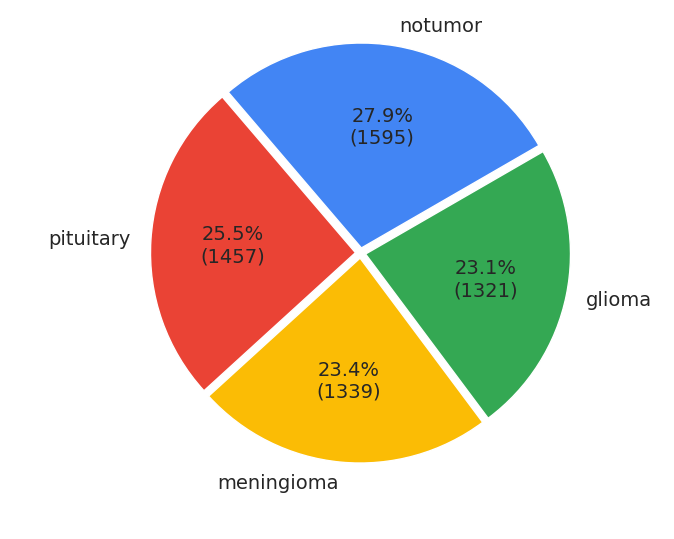
\includegraphics[width=0.45\textwidth]{class distribution.PNG}
    \caption{Pie chart of class distribution within Brain Tumor MRI dataset.}
    \label{fig:piechart}
\end{figure}

The pre-trained B16 ViT model produced by Google is a rather typical ViT. The B16 ViT model takes in a flattened or linear positionally-embedded patched image that gets fed through a multi-head attention layer initially then into two fully connected layers and finally into a mutli-layer perceptron (MLP) head that performs the classification. Furthermore, there are residual connections between the input layer and the output of the multi-head attention layer as well as from the output of the multi-head attention layer to the input of the MLP to address potential vanishing/exploding gradients. Furthermore, to distinguish between the typical transformer model and ViTs, one must note that ViTs do not employ a transformer decoder but rather only encode the information and performing classification on this encoded vector.

Rather than update the size of the input layer, we adjusted our image resolutions to 224x224 as is standard practice with this model and also due to the fact that the images came in various resolutions as they are from different datasets. Furthermore, we employed the Adam optimizer along with a loss function of cross entropy at a learning rate of 1e$^{-3}$ and we set the torch and torch.cuda random seed value to 42. The pre-trained B16 ViT also expects three color channels; however, given that our MRI images are in grey scale, we adjusted the model's input layer to accept one color channel. Furthermore, we adjusted the shape of the MLP classification head for four classes. Finally, we froze the model in all layers except in the MLP to fine tune classification and to take advantage of the pre-trained multi-head attention block.

To summarize the flow of information through BrainViT: the first step is to rescale the images into an image 224 pixels by 224 pixels which is then patched by 16 pixel by 16 pixel squares which creates 196 sub-image matrices. From here, the image is flattened and given a positional embedding which allows the transformer model to be aware of how the pieces of the image interact spatially. This is how ViTs are capable of capturing both long-range and short-range dependencies. The positionally encoded vector of image data then flows through a normalization layer where the pixel values are standardized to the range [0, 1] and fed into the mutli-head attention layer. The multi-head attention layer then pushes the data through an attention mechanism several times in parallel to process the entire image in one go. From the output of the multi-head attention layer, the initial image information is re-encoded into the output to decrease chances of vanishing gradients via the residual connection previously noted. The data is then fed through another normalization layer and finally into the MLP where classification occurs via GeLu activation for both multi-label and multi-class classification for the potential of an individual having multiple tumor types. The GeLu function also allows for capturing of non-linear relationships. Finally, the classification vector has an argmax function applied to it to receive the final classification(s).  

\begin{figure}[h]
    \centering
    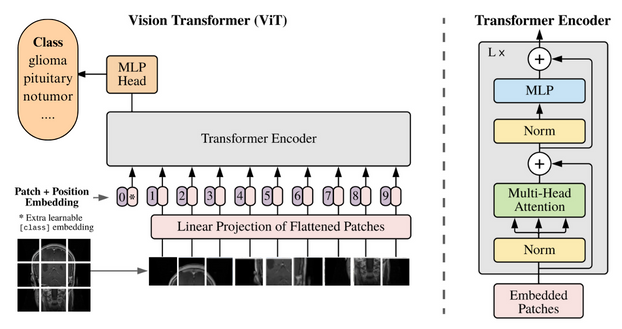
\includegraphics[width=0.45\textwidth]{arch.png}
    \caption{BrainViT Architecture w/ example patched MRI image to a linear projection.}
    \label{fig:1}
\end{figure}

\begin{figure}[h]
    \centering
    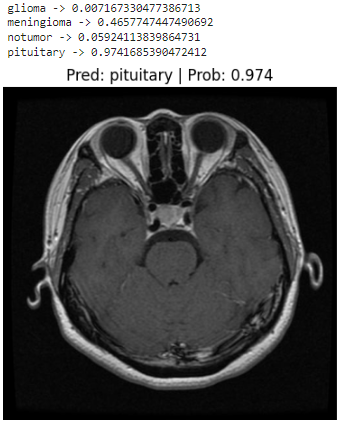
\includegraphics[width=0.45\textwidth]{example output.PNG}
    \caption{BrainViT example output and classification.}
    \label{fig:output}
\end{figure}

\section{Results}
We trained the model for 50 epochs at which point we were observing a training accuracy of 98.64\% along with a testing accuracy of 95.20\%. Which, when compared against a typical CNN that trained for 357 epochs, only achieved an accuracy of 92.5\% which was produced by Ramez Samy on Kaggle$^{[7]}$. When one considers the fact that the CNN model has to train for 10x more epochs along with the lower performance - one can quickly see the value in using a ViT over other deep learning techniques. Furthermore, a larger VGG model produced on Kaggle by Kevin Tian which employed the well known VGG 19 with adjusted architecture for the task achieved accuracies in the 97\% range with 179 epochs$^{[8]}$. Both of these models produced by Samy and Tian employed the usage of the same dataset as we did. Finally, to cross validate the results we were seeing from other models, we used an adjusted architecture of ResNet50 (a CNN with residual connections) with 50 training epochs and saw an accuracy of about 80\%. The ResNet50 model also had a much more noisy approach on the loss and accuracy during training which can be seen in figure 4.

\begin{figure}[htbp]
    \centering
    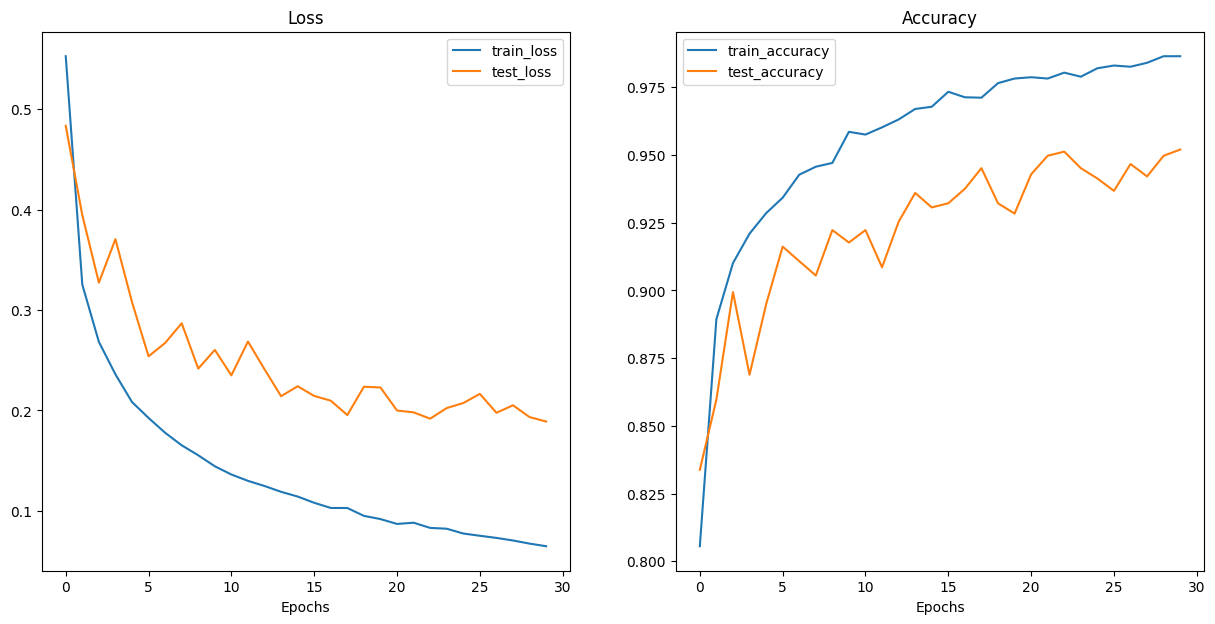
\includegraphics[width=0.45\textwidth]{graph.png}
    \caption{Plot of loss function and accuracy over initial 30 training epochs.}
    \label{fig:2}
\end{figure}

\begin{figure}[htbp]
    \centering
    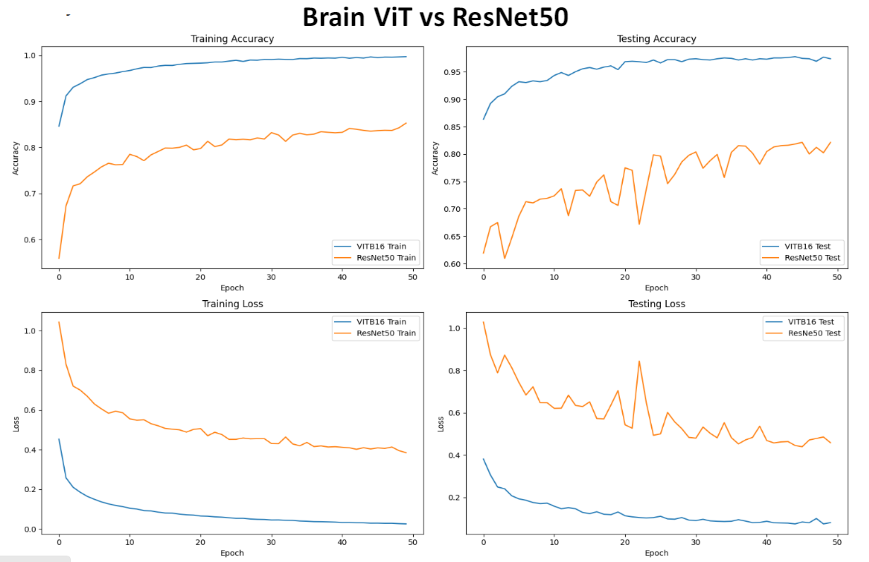
\includegraphics[width=0.45\textwidth]{resnet versus brainvit.PNG}
    \caption{Plot of loss and accuracy of BrainViT versus ResNet50 over final 50 training epochs.}
    \label{fig:3}
\end{figure}

\begin{figure}[htbp]
    \centering
    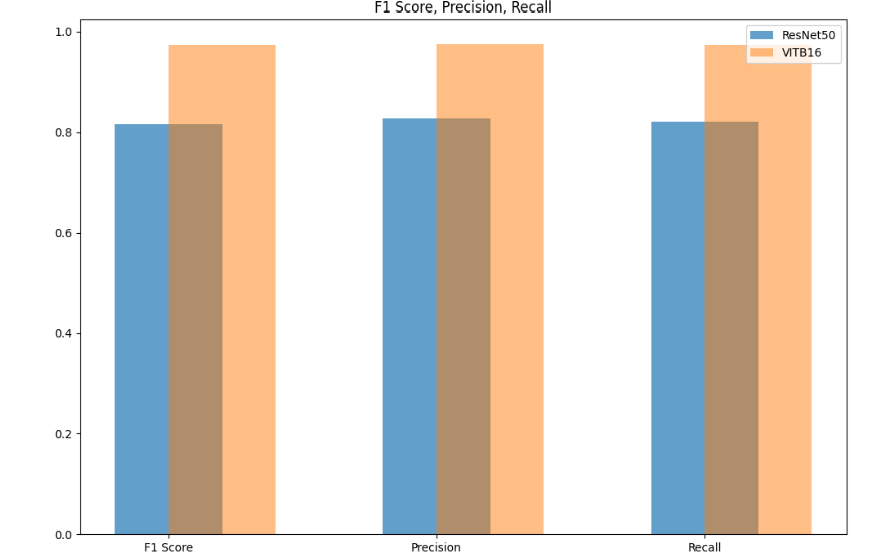
\includegraphics[width=0.45\textwidth]{resnet versus brainvit2.PNG}
    \caption{Bar graph of ResNet50 versus BrainViT F1 score, precision, and recall.}
    \label{fig:4}
\end{figure}

\begin{table}[htbp]
    \centering
    \caption{Precision, Recall, and F1 Score by Class}
    \label{tab:example_with_headers}
    \begin{tabular}{|c|c|c|c|c|}
        \hline
        \textbf{Class} & \textbf{Precision} & \textbf{Recall} & \textbf{F1 Score} & \textbf{Avg. Accuracy}\\ 
        \hline
        Glioma & 0.97 & 0.92 & 0.95 & N/A\\ 
        Meningioma & 0.86 & 0.98 & 0.91 & N/A \\ 
        Pituitary & 0.99 & 0.99 & 0.99 & N/A\\
        Not Tumor & 1.00 & 0.93 & 0.96 & N/A\\
        Average Accuracy & N/A & N/A & N/A & 0.95 \\
        \hline
    \end{tabular}
\end{table}

\begin{figure}[h]
    \centering
    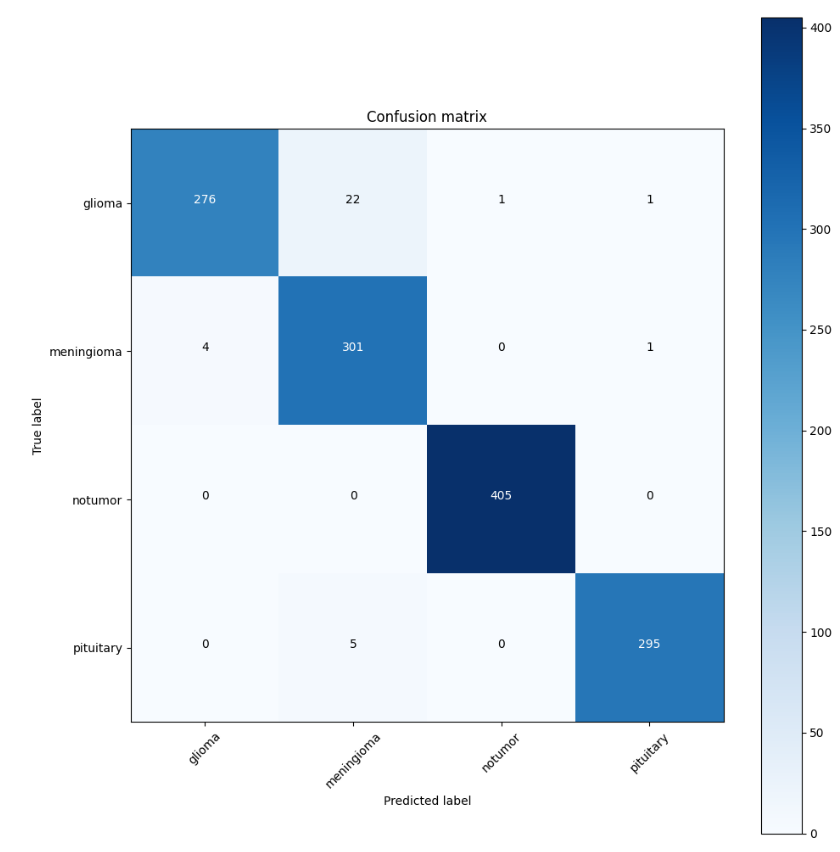
\includegraphics[width=0.45\textwidth]{results cm.PNG}
    \caption{BrainViT confusion matrix of results throughout classes.}
    \label{fig:cm}
\end{figure}

\section{Discussion}
BrainViT is quite easy to use from a medical practitioners point of view - once the MRI image has been loaded into the model, BrainViT will accurately classify the image with the assumption that the tumor type is within the trained pathology list. If the disease from the image is not within the trained pathology list then results may vary. Furthermore, given a large enough dataset and access to high performance computing, BrainViT can quickly be trained to identify other brain pathologies. For access to the pre-trained BrainViT model navigate to https://github.com/vivekkiran/BrainViT.

BrainViT provides medical practitioners a highly reliable, quick, and accurate diagnosis methodology. Typically, to make a diagnosis, one would have to have multiple tests run such as imaging, biopsies, and blood tests, all of which would have to be interpreted by someone how has gone through many years of schooling and training to be able to make a confident diagnosis. Comparing this to BrainViT which trained in under one month on a relatively small dataset, BrainViT is the clear victor and will see higher accuracy and confidence in diagnosis with larger datasets and longer training times.

BrainViT was able to produce high accuracy classification with a relatively small training time given how many epochs ViT models are typically trained for. From scratch ViTs with randomized weights typically require millions of images and thousands of epochs to be able to approach confident results. This reality was avoided in BrainViT by using pre-trained multi-head attention layer weights that do most of the heavy lifting. With that being said, given a large dataset - to avoid over fitting of any particular pathology - along with access to high performance computing (HPC), one would likely see much higher accuracy. Furthermore, given a dataset with more classes, we believe the model will likely perform well in this case as well given that the B16 ViT model has been known to be able to perform well on the ImageNet 1000 class dataset.

Having shown proof of concept, the next step will be to produce a similar ViT architecture in the Julia programming language which has seen great success, performance, and speed within the machine learning/data science field. After having produced this model we will be able to train it on a larger dataset with more classes on HPC at the University of South Dakota. Furthermore, we are conducting research into utilizing vision mamba which is a competing architecture with ViTs. Vision mamba uses state space models to efficiently learn visual relationships in comparison with ViTs using transformer blocks with an emphasis on the multi-head attention layer.

\section{Conlcusion}
BrainViT showed promising results from a pre-trained B16 ViT model with slight adaptations to the architecture showing weighted - across all classes - average accuracy of 95.20\% on a relatively small training time and dataset. The next step will be to produce a "from scratch" Julia BrainViT to fine tune performance increase efficiency along with gathering a larger dataset with more classes to allow BrainViT to be applicable to more disease classification. Furthermore, these results from a "from scratch" Julia model will be compared against BrainViT and vision mamba results.

\section*{Acknowledgment}
We thank the University of South Dakota for granting us HPC access during the summer of 2024 to train our Julia BrainViT. Further thanks to Dr. Rodrgiue Rizk and Dr. K.C. Santosh for providing support and guidance during this project. Finally, we thank to the 2AI volunteer team at the University of South Dakota for collaborating and assisting with idea development and providing feedback.

\begin{thebibliography}{00}
\bibitem{b1} A. Vaswani et al., “Attention is all you need,” in Advances in Neural Information Processing Systems, 2017.
\bibitem{b2} M. Nickparvar. "Brain tumor MRI dataset," in Kaggle, 2021. 
\bibitem{b3} PyTorch, "ViT-B/16: Vision Transformer with BERT-style tokens," PyTorch torchvision Library.
\bibitem{b4} J. Cheng, "Brain tumor dataset," 2017.
\bibitem{b5} J. Sarta, "Brain tumor classification (MRI)," in Kaggle, 2020.
\bibitem{b6} A. Hamada, "Br35H:: Brain tumor detection 2021," in Kaggle, 2020.
\bibitem{b7} R. Samy, "Brain tumor using CNN," in Kaggle, 2024.
\bibitem{b8} K. Tian, "Brain tumor type classification - VGG-19," in Kaggle, 2024.
\bibitem{b9} A. Dosovitskiy et al., “AN IMAGE IS WORTH 16X16 WORDS: TRANSFORMERS FOR IMAGE RECOGNITION AT SCALE,” in ICLR 2021 - 9th International Conference on Learning Representations, 2021.

Related Work:
\bibitem{b10} Z. Xia, X. Pan, S. Song, L. E. Li, and G. Huang, “Vision Transformer with Deformable Attention,” in Proceedings of the IEEE Computer Society Conference on Computer Vision and Pattern Recognition, 2022. doi: 10.1109/CVPR52688.2022.00475.
\bibitem{b11} W. Sun et al., “Vicinity Vision Transformer,” IEEE Trans Pattern Anal Mach Intell, vol. 45, no. 10, 2023, doi: 10.1109/TPAMI.2023.3285569.
\bibitem{b12} X. Mao et al., “Towards Robust Vision Transformer,” in Proceedings of the IEEE Computer Society Conference on Computer Vision and Pattern Recognition, 2022. doi: 10.1109/CVPR52688.2022.01173.
\end{thebibliography}

\end{document}
